\chapter{博弈论}

本章重点讨论不含随机因素的双人博弈。目标是判断是否存在一种策略，使我们无论对手如何行动都能获胜，并在存在时找出该策略。

这类博弈存在一套通用理论，可以用\key{Nim 理论}进行分析。首先研究玩家从若干堆中取走木棍的简单博弈，再把其中的策略推广到其他博弈。

\section{博弈状态}

考虑这样一个博弈：初始有一堆 $n$ 根木棍，玩家 $A$、$B$ 轮流行动，由 $A$ 先手。每次必须从堆中取走 1、2 或 3 根木棍，取走最后一根木棍的玩家获胜。

例如，当 $n=10$ 时，博弈可能按如下过程进行：
\begin{itemize}[noitemsep]
\item 玩家 $A$ 取走 2 根（剩余 8 根）。
\item 玩家 $B$ 取走 3 根（剩余 5 根）。
\item 玩家 $A$ 取走 1 根（剩余 4 根）。
\item 玩家 $B$ 取走 2 根（剩余 2 根）。
\item 玩家 $A$ 取走 2 根并获胜。
\end{itemize}

该博弈包含状态 $0,1,2,\ldots,n$，状态编号表示剩余木棍数量。

\subsubsection{必胜态与必败态}

\index{winning state}
\index{losing state}

\key{必胜态}是指当前玩家采用最优策略即可获胜的状态；\key{必败态}是指对手采用最优策略时当前玩家必定失败的状态。博弈中的每个状态都可以分类为必胜态或必败态。

在上述博弈中，状态 0 显然是必败态，因为当前玩家无法行动。状态 1、2、3 是必胜态，因为可以分别取走 1、2、3 根并立即获胜。状态 4 则是必败态，因为任何行动都会把局面转移到对手的必胜态。

更一般地说，如果存在一步行动能从当前状态转移到必败态，那么当前状态就是必胜态；否则，当前状态就是必败态。利用这一结论，我们可以从无路可走的必败态开始，对博弈的所有状态进行分类。

上述博弈的状态 $0 \ldots 15$ 可分类如下（$W$ 表示必胜态，$L$ 表示必败态）：
\begin{center}
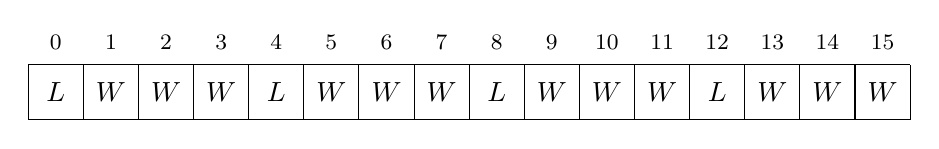
\begin{tikzpicture}[scale=0.7]
\draw (0,0) grid (16,1);

\node at (0.5,0.5) {$L$};
\node at (1.5,0.5) {$W$};
\node at (2.5,0.5) {$W$};
\node at (3.5,0.5) {$W$};
\node at (4.5,0.5) {$L$};
\node at (5.5,0.5) {$W$};
\node at (6.5,0.5) {$W$};
\node at (7.5,0.5) {$W$};
\node at (8.5,0.5) {$L$};
\node at (9.5,0.5) {$W$};
\node at (10.5,0.5) {$W$};
\node at (11.5,0.5) {$W$};
\node at (12.5,0.5) {$L$};
\node at (13.5,0.5) {$W$};
\node at (14.5,0.5) {$W$};
\node at (15.5,0.5) {$W$};

\footnotesize
\node at (0.5,1.4) {$0$};
\node at (1.5,1.4) {$1$};
\node at (2.5,1.4) {$2$};
\node at (3.5,1.4) {$3$};
\node at (4.5,1.4) {$4$};
\node at (5.5,1.4) {$5$};
\node at (6.5,1.4) {$6$};
\node at (7.5,1.4) {$7$};
\node at (8.5,1.4) {$8$};
\node at (9.5,1.4) {$9$};
\node at (10.5,1.4) {$10$};
\node at (11.5,1.4) {$11$};
\node at (12.5,1.4) {$12$};
\node at (13.5,1.4) {$13$};
\node at (14.5,1.4) {$14$};
\node at (15.5,1.4) {$15$};
\end{tikzpicture}
\end{center}

这个博弈很容易分析：当 $k$ 能被 4 整除时，状态 $k$ 是必败态；否则是必胜态。最优策略是每次行动后都让堆中剩余木棍数能被 4 整除。最终木棍会全部取完，而对手失败。

当然，该策略要求轮到我们行动时，木棍数\emph{不能}被 4 整除。若能被 4 整除，我们便无计可施；只要对手采用最优策略，他就会获胜。

\subsubsection{状态图}

现在考虑另一种木棍博弈。在状态 $k$，允许取走任意数量 $x$ 的木棍，其中 $x<k$ 且 $x$ 整除 $k$。例如，在状态 8 可以取走 1、2 或 4 根，而在状态 7 只能取走 1 根。

下图把该博弈的状态 $1 \ldots 9$ 表示为一张\key{状态图}，图中的节点表示状态，边表示状态之间的行动：

\begin{center}
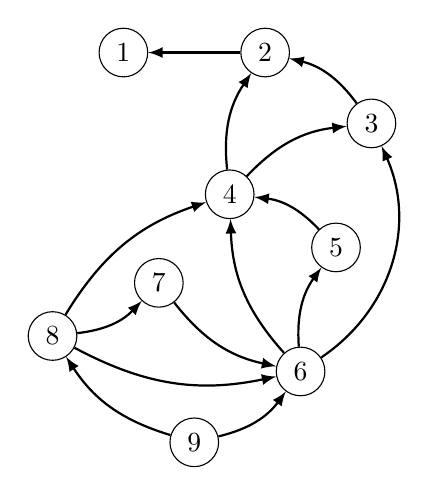
\begin{tikzpicture}[scale=0.9]
\node[draw, circle] (1) at (0,0) {$1$};
\node[draw, circle] (2) at (2,0) {$2$};
\node[draw, circle] (3) at (3.5,-1) {$3$};
\node[draw, circle] (4) at (1.5,-2) {$4$};
\node[draw, circle] (5) at (3,-2.75) {$5$};
\node[draw, circle] (6) at (2.5,-4.5) {$6$};
\node[draw, circle] (7) at (0.5,-3.25) {$7$};
\node[draw, circle] (8) at (-1,-4) {$8$};
\node[draw, circle] (9) at (1,-5.5) {$9$};

\path[draw,thick,->,>=latex] (2) -- (1);
\path[draw,thick,->,>=latex] (3) edge [bend right=20] (2);
\path[draw,thick,->,>=latex] (4) edge [bend left=20] (2);
\path[draw,thick,->,>=latex] (4) edge [bend left=20] (3);
\path[draw,thick,->,>=latex] (5) edge [bend right=20] (4);
\path[draw,thick,->,>=latex] (6) edge [bend left=20] (5);
\path[draw,thick,->,>=latex] (6) edge [bend left=20] (4);
\path[draw,thick,->,>=latex] (6) edge [bend right=40] (3);
\path[draw,thick,->,>=latex] (7) edge [bend right=20] (6);
\path[draw,thick,->,>=latex] (8) edge [bend right=20] (7);
\path[draw,thick,->,>=latex] (8) edge [bend right=20] (6);
\path[draw,thick,->,>=latex] (8) edge [bend left=20] (4);
\path[draw,thick,->,>=latex] (9) edge [bend left=20] (8);
\path[draw,thick,->,>=latex] (9) edge [bend right=20] (6);
\end{tikzpicture}
\end{center}

该博弈的最终状态总是状态 1；由于此时没有合法行动，它是必败态。状态 $1 \ldots 9$ 的分类如下：

\begin{center}
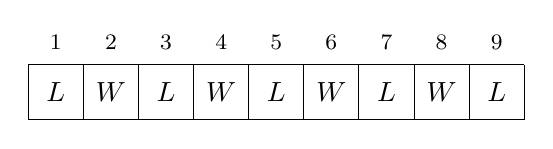
\begin{tikzpicture}[scale=0.7]
\draw (1,0) grid (10,1);

\node at (1.5,0.5) {$L$};
\node at (2.5,0.5) {$W$};
\node at (3.5,0.5) {$L$};
\node at (4.5,0.5) {$W$};
\node at (5.5,0.5) {$L$};
\node at (6.5,0.5) {$W$};
\node at (7.5,0.5) {$L$};
\node at (8.5,0.5) {$W$};
\node at (9.5,0.5) {$L$};

\footnotesize
\node at (1.5,1.4) {$1$};
\node at (2.5,1.4) {$2$};
\node at (3.5,1.4) {$3$};
\node at (4.5,1.4) {$4$};
\node at (5.5,1.4) {$5$};
\node at (6.5,1.4) {$6$};
\node at (7.5,1.4) {$7$};
\node at (8.5,1.4) {$8$};
\node at (9.5,1.4) {$9$};
\end{tikzpicture}
\end{center}

令人意外的是，在这个博弈中，所有偶数状态都是必胜态，所有奇数状态都是必败态。

\section{Nim 博弈}

\index{nim game}

\key{Nim 博弈}是一种简单却在博弈论中十分重要的博弈，因为许多其他博弈都可以采用相同的策略。我们先研究 Nim 博弈，再把它的策略推广到其他博弈。

该博弈中有 $n$ 个堆，每堆包含若干根木棍。两名玩家轮流行动；每回合选择一个仍有木棍的堆，并从中取走任意数量的木棍。取走最后一根木棍的玩家获胜。

其状态形如 $[x_1,x_2,\ldots,x_n]$，其中 $x_k$ 表示第 $k$ 堆中的木棍数。例如，$[10,12,5]$ 表示有三堆木棍，数量分别为 10、12 和 5。状态 $[0,0,\ldots,0]$ 是必败态，因为此时无法再取走木棍；它也总是终止状态。

\subsubsection{分析}
\index{nim sum}

事实证明，只需计算\key{Nim 和} $s = x_1 \oplus x_2 \oplus \cdots \oplus x_n$，就能轻易判定任意 Nim 状态，其中 $\oplus$ 表示异或运算\footnote{Nim 博弈的最优策略由 C. L. Bouton 于 1901 年发表 \cite{bou01}。}。Nim 和为 0 的状态是必败态，其余状态都是必胜态。例如，$[10,12,5]$ 的 Nim 和为 $10 \oplus 12 \oplus 5 = 3$，所以它是必胜态。

这种异或和与该博弈究竟有何联系？考察状态改变时异或和如何变化即可说明这一点。

\textit{必败态：}
终止状态 $[0,0,\ldots,0]$ 是必败态，其 Nim 和如预期为 0。在其他必败态中，任何行动都会到达必胜态，因为单个 $x_k$ 改变时 Nim 和也会改变，行动后的 Nim 和因而不再为 0。

\textit{必胜态：}
如果存在一个堆 $k$ 满足 $x_k \oplus s < x_k$，就可以转移到必败态。此时从第 $k$ 堆取走一些木棍，使其剩下 $x_k \oplus s$ 根，即可到达必败态。这样的堆一定存在：在 $s$ 的最高位 1 所在位置，$x_k$ 也有一个二进制位 1。

以状态 $[10,12,5]$ 为例。它的 Nim 和为 3，因此是必胜态，所以必然存在一步行动能够到达必败态。下面找出这样的一步。

该状态的 Nim 和如下：

\begin{center}
\begin{tabular}{r|r}
10 & \texttt{1010} \\
12 & \texttt{1100} \\
5 & \texttt{0101} \\
\hline
3 & \texttt{0011} \\
\end{tabular}
\end{center}

在此例中，Nim 和最高位 1 所在的位置上，只有包含 10 根木棍的堆具有二进制位 1：

\begin{center}
\begin{tabular}{r|r}
10 & \texttt{10\underline{1}0} \\
12 & \texttt{1100} \\
5 & \texttt{0101} \\
\hline
3 & \texttt{00\underline{1}1} \\
\end{tabular}
\end{center}

该堆的新大小必须为 $10 \oplus 3 = 9$，所以只需取走一根木棍。此后状态变为 $[9,12,5]$，它是必败态：

\begin{center}
\begin{tabular}{r|r}
9 & \texttt{1001} \\
12 & \texttt{1100} \\
5 & \texttt{0101} \\
\hline
0 & \texttt{0000} \\
\end{tabular}
\end{center}

\subsubsection{反常玩法}

\index{misère game}

在\key{反常玩法}中，目标恰好相反：取走最后一根木棍的玩家失败。事实证明，反常 Nim 博弈的最优玩法与标准 Nim 博弈几乎相同。

基本思路是先按标准玩法进行反常博弈，只在临近结束时改变策略。当下一步行动后每个堆至多只剩一根木棍时，就切换到新策略。

在标准玩法中，应使行动后恰有一根木棍的堆数为偶数；而在反常玩法中，应使这样的堆数为奇数。

该策略之所以成立，是因为博弈中总会出现需要切换策略的状态，而且它是必胜态：此时恰好只有一个堆含有多于一根木棍，因此 Nim 和不为 0。

\section{Sprague--Grundy 定理}

\index{Sprague–Grundy theorem}

\key{Sprague--Grundy 定理}\footnote{该定理由 R. Sprague \cite{spr35} 和 P. M. Grundy \cite{gru39} 分别独立发现。}把 Nim 博弈的策略推广到满足以下条件的所有博弈：

\begin{itemize}[noitemsep]
\item 两名玩家轮流行动。
\item 博弈由若干状态组成，某一状态下可采取的行动与轮到哪名玩家无关。
\item 当某名玩家无法行动时，博弈结束。
\item 博弈必定会在有限步内结束。
\item 玩家完全了解各状态与合法行动，博弈中不存在随机因素。
\end{itemize}
核心思想是为每个博弈状态计算一个 Grundy 数，它对应于 Nim 博弈中某一堆的木棍数。知道所有状态的 Grundy 数后，就能像 Nim 博弈一样处理该博弈。

\subsubsection{Grundy 数}

\index{Grundy number}
\index{mex function}

一个博弈状态的\key{Grundy 数}为
\[\textrm{mex}(\{g_1,g_2,\ldots,g_n\}),\]
其中 $g_1,g_2,\ldots,g_n$ 是所有可达状态的 Grundy 数，而 mex 函数返回不在该集合中的最小非负整数。例如，$\textrm{mex}(\{0,1,3\})=2$。若某状态没有合法行动，其 Grundy 数为 0，因为 $\textrm{mex}(\emptyset)=0$。

例如，在下面的状态图中
\begin{center}
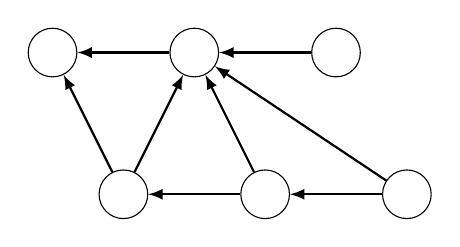
\begin{tikzpicture}[scale=0.9]
\node[draw, circle] (1) at (0,0) {\phantom{0}};
\node[draw, circle] (2) at (2,0) {\phantom{0}};
\node[draw, circle] (3) at (4,0) {\phantom{0}};
\node[draw, circle] (4) at (1,-2) {\phantom{0}};
\node[draw, circle] (5) at (3,-2) {\phantom{0}};
\node[draw, circle] (6) at (5,-2) {\phantom{0}};

\path[draw,thick,->,>=latex] (2) -- (1);
\path[draw,thick,->,>=latex] (3) -- (2);
\path[draw,thick,->,>=latex] (5) -- (4);
\path[draw,thick,->,>=latex] (6) -- (5);
\path[draw,thick,->,>=latex] (4) -- (1);
\path[draw,thick,->,>=latex] (4) -- (2);
\path[draw,thick,->,>=latex] (5) -- (2);
\path[draw,thick,->,>=latex] (6) -- (2);
\end{tikzpicture}
\end{center}
各状态的 Grundy 数如下：
\begin{center}
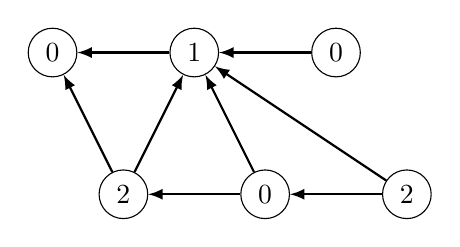
\begin{tikzpicture}[scale=0.9]
\node[draw, circle] (1) at (0,0) {0};
\node[draw, circle] (2) at (2,0) {1};
\node[draw, circle] (3) at (4,0) {0};
\node[draw, circle] (4) at (1,-2) {2};
\node[draw, circle] (5) at (3,-2) {0};
\node[draw, circle] (6) at (5,-2) {2};

\path[draw,thick,->,>=latex] (2) -- (1);
\path[draw,thick,->,>=latex] (3) -- (2);
\path[draw,thick,->,>=latex] (5) -- (4);
\path[draw,thick,->,>=latex] (6) -- (5);
\path[draw,thick,->,>=latex] (4) -- (1);
\path[draw,thick,->,>=latex] (4) -- (2);
\path[draw,thick,->,>=latex] (5) -- (2);
\path[draw,thick,->,>=latex] (6) -- (2);
\end{tikzpicture}
\end{center}
必败态的 Grundy 数为 0，必胜态的 Grundy 数为正数。

一个状态的 Grundy 数对应于 Nim 博弈中一堆木棍的数量。若 Grundy 数为 0，则只能转移到 Grundy 数为正数的状态；若 Grundy 数为 $x>0$，则可以转移到 Grundy 数分别为 $0,1,\ldots,x-1$ 的状态。

例如，考虑一个玩家在迷宫中移动棋子的博弈。迷宫中的每个方格要么是可通行区域，要么是墙。每回合，玩家必须把棋子向左或向上移动若干格。完成最后一次移动的玩家获胜。

下图给出一种可能的初始状态，其中 @ 表示棋子，* 表示它可以移动到的方格。

\begin{center}
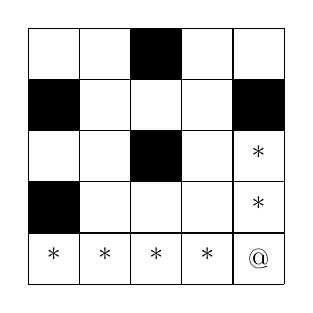
\begin{tikzpicture}[scale=.65]
  \begin{scope}
    \fill [color=black] (0, 1) rectangle (1, 2);
    \fill [color=black] (0, 3) rectangle (1, 4);
    \fill [color=black] (2, 2) rectangle (3, 3);
    \fill [color=black] (2, 4) rectangle (3, 5);
    \fill [color=black] (4, 3) rectangle (5, 4);

    \draw (0, 0) grid (5, 5);
    
    \node at (4.5,0.5) {@};
    \node at (3.5,0.5) {*};
    \node at (2.5,0.5) {*};
    \node at (1.5,0.5) {*};
    \node at (0.5,0.5) {*};
    \node at (4.5,1.5) {*};
    \node at (4.5,2.5) {*};
    
  \end{scope}
\end{tikzpicture}
\end{center}

该博弈的状态是迷宫中所有可通行的方格。在上述迷宫中，各状态的 Grundy 数如下：

\begin{center}
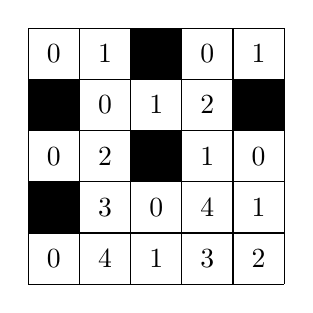
\begin{tikzpicture}[scale=.65]
  \begin{scope}
    \fill [color=black] (0, 1) rectangle (1, 2);
    \fill [color=black] (0, 3) rectangle (1, 4);
    \fill [color=black] (2, 2) rectangle (3, 3);
    \fill [color=black] (2, 4) rectangle (3, 5);
    \fill [color=black] (4, 3) rectangle (5, 4);

    \draw (0, 0) grid (5, 5);
    
    \node at (0.5,4.5) {0};
    \node at (1.5,4.5) {1};
    \node at (2.5,4.5) {};
    \node at (3.5,4.5) {0};
    \node at (4.5,4.5) {1};

    \node at (0.5,3.5) {};
    \node at (1.5,3.5) {0};
    \node at (2.5,3.5) {1};
    \node at (3.5,3.5) {2};
    \node at (4.5,3.5) {};

    \node at (0.5,2.5) {0};
    \node at (1.5,2.5) {2};
    \node at (2.5,2.5) {};
    \node at (3.5,2.5) {1};
    \node at (4.5,2.5) {0};

    \node at (0.5,1.5) {};
    \node at (1.5,1.5) {3};
    \node at (2.5,1.5) {0};
    \node at (3.5,1.5) {4};
    \node at (4.5,1.5) {1};

    \node at (0.5,0.5) {0};
    \node at (1.5,0.5) {4};
    \node at (2.5,0.5) {1};
    \node at (3.5,0.5) {3};
    \node at (4.5,0.5) {2};
  \end{scope}
\end{tikzpicture}
\end{center}

因此，迷宫博弈中的每个状态都对应于 Nim 博弈中的一堆木棍。例如，右下角方格的 Grundy 数为 2，所以它是必胜态。向左移动四格或向上移动两格，都可以到达必败态并赢得博弈。

注意，与原始 Nim 博弈不同，这里可能转移到 Grundy 数比当前状态更大的状态。不过，对手总能选择一步行动抵消这种转移，因此无法从必败态中逃脱。

\subsubsection{子博弈}

下面假设整个博弈由若干子博弈组成。每回合，玩家先选择一个子博弈，再在其中采取一步行动。当所有子博弈都无法行动时，整个博弈结束。

此时，整个博弈的 Grundy 数等于各子博弈 Grundy 数的 Nim 和。只需计算所有子博弈的 Grundy 数及其 Nim 和，就可以像处理 Nim 博弈一样进行游戏。

例如，考虑一个由三个迷宫组成的博弈。每回合，玩家选择一个迷宫，并在其中移动棋子。假设初始状态如下：

\begin{center}
\begin{tabular}{ccc}
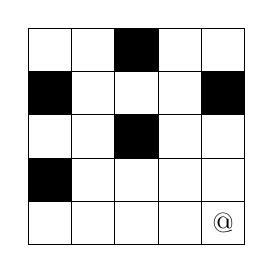
\begin{tikzpicture}[scale=.55]
  \begin{scope}
    \fill [color=black] (0, 1) rectangle (1, 2);
    \fill [color=black] (0, 3) rectangle (1, 4);
    \fill [color=black] (2, 2) rectangle (3, 3);
    \fill [color=black] (2, 4) rectangle (3, 5);
    \fill [color=black] (4, 3) rectangle (5, 4);

    \draw (0, 0) grid (5, 5);

    \node at (4.5,0.5) {@};

    \end{scope}
\end{tikzpicture}
&
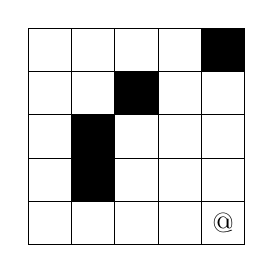
\begin{tikzpicture}[scale=.55]
  \begin{scope}
    \fill [color=black] (1, 1) rectangle (2, 3);
    \fill [color=black] (2, 3) rectangle (3, 4);
    \fill [color=black] (4, 4) rectangle (5, 5);

    \draw (0, 0) grid (5, 5);
    
    \node at (4.5,0.5) {@};

  \end{scope}
\end{tikzpicture}
&
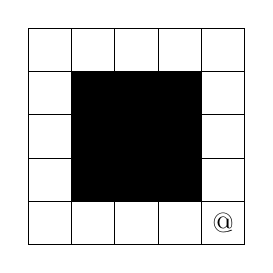
\begin{tikzpicture}[scale=.55]
  \begin{scope}
    \fill [color=black] (1, 1) rectangle (4, 4);

    \draw (0, 0) grid (5, 5);
    
    \node at (4.5,0.5) {@};
  \end{scope}
\end{tikzpicture}
\end{tabular}
\end{center}

三个迷宫各状态的 Grundy 数如下：

\begin{center}
\begin{tabular}{ccc}
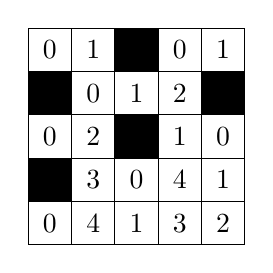
\begin{tikzpicture}[scale=.55]
  \begin{scope}
    \fill [color=black] (0, 1) rectangle (1, 2);
    \fill [color=black] (0, 3) rectangle (1, 4);
    \fill [color=black] (2, 2) rectangle (3, 3);
    \fill [color=black] (2, 4) rectangle (3, 5);
    \fill [color=black] (4, 3) rectangle (5, 4);

    \draw (0, 0) grid (5, 5);

    \node at (0.5,4.5) {0};
    \node at (1.5,4.5) {1};
    \node at (2.5,4.5) {};
    \node at (3.5,4.5) {0};
    \node at (4.5,4.5) {1};

    \node at (0.5,3.5) {};
    \node at (1.5,3.5) {0};
    \node at (2.5,3.5) {1};
    \node at (3.5,3.5) {2};
    \node at (4.5,3.5) {};

    \node at (0.5,2.5) {0};
    \node at (1.5,2.5) {2};
    \node at (2.5,2.5) {};
    \node at (3.5,2.5) {1};
    \node at (4.5,2.5) {0};

    \node at (0.5,1.5) {};
    \node at (1.5,1.5) {3};
    \node at (2.5,1.5) {0};
    \node at (3.5,1.5) {4};
    \node at (4.5,1.5) {1};

    \node at (0.5,0.5) {0};
    \node at (1.5,0.5) {4};
    \node at (2.5,0.5) {1};
    \node at (3.5,0.5) {3};
    \node at (4.5,0.5) {2};
    \end{scope}
\end{tikzpicture}
&
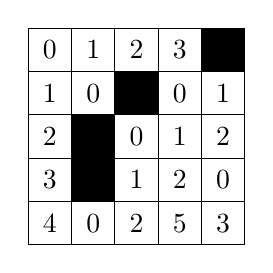
\begin{tikzpicture}[scale=.55]
  \begin{scope}
    \fill [color=black] (1, 1) rectangle (2, 3);
    \fill [color=black] (2, 3) rectangle (3, 4);
    \fill [color=black] (4, 4) rectangle (5, 5);

    \draw (0, 0) grid (5, 5);

    \node at (0.5,4.5) {0};
    \node at (1.5,4.5) {1};
    \node at (2.5,4.5) {2};
    \node at (3.5,4.5) {3};
    \node at (4.5,4.5) {};

    \node at (0.5,3.5) {1};
    \node at (1.5,3.5) {0};
    \node at (2.5,3.5) {};
    \node at (3.5,3.5) {0};
    \node at (4.5,3.5) {1};

    \node at (0.5,2.5) {2};
    \node at (1.5,2.5) {};
    \node at (2.5,2.5) {0};
    \node at (3.5,2.5) {1};
    \node at (4.5,2.5) {2};

    \node at (0.5,1.5) {3};
    \node at (1.5,1.5) {};
    \node at (2.5,1.5) {1};
    \node at (3.5,1.5) {2};
    \node at (4.5,1.5) {0};

    \node at (0.5,0.5) {4};
    \node at (1.5,0.5) {0};
    \node at (2.5,0.5) {2};
    \node at (3.5,0.5) {5};
    \node at (4.5,0.5) {3};
  \end{scope}
\end{tikzpicture}
&
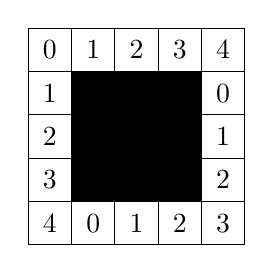
\begin{tikzpicture}[scale=.55]
  \begin{scope}
    \fill [color=black] (1, 1) rectangle (4, 4);

    \draw (0, 0) grid (5, 5);

    \node at (0.5,4.5) {0};
    \node at (1.5,4.5) {1};
    \node at (2.5,4.5) {2};
    \node at (3.5,4.5) {3};
    \node at (4.5,4.5) {4};

    \node at (0.5,3.5) {1};
    \node at (1.5,3.5) {};
    \node at (2.5,3.5) {};
    \node at (3.5,3.5) {};
    \node at (4.5,3.5) {0};

    \node at (0.5,2.5) {2};
    \node at (1.5,2.5) {};
    \node at (2.5,2.5) {};
    \node at (3.5,2.5) {};
    \node at (4.5,2.5) {1};

    \node at (0.5,1.5) {3};
    \node at (1.5,1.5) {};
    \node at (2.5,1.5) {};
    \node at (3.5,1.5) {};
    \node at (4.5,1.5) {2};

    \node at (0.5,0.5) {4};
    \node at (1.5,0.5) {0};
    \node at (2.5,0.5) {1};
    \node at (3.5,0.5) {2};
    \node at (4.5,0.5) {3};
  \end{scope}
\end{tikzpicture}
\end{tabular}
\end{center}

在初始状态中，三个 Grundy 数的 Nim 和为 $2 \oplus 3 \oplus 3 = 2$，因此先手可以获胜。一种最优行动是在第一个迷宫中向上移动两格，使 Nim 和变为 $0 \oplus 3 \oplus 3 = 0$。

\subsubsection{Grundy 博弈}

有时，博弈中的一步行动会把原博弈分成彼此独立的若干子博弈。此时，原博弈的 Grundy 数为

\[\textrm{mex}(\{g_1, g_2, \ldots, g_n \}),\]
其中 $n$ 是合法行动的数量，并且
\[g_k = a_{k,1} \oplus a_{k,2} \oplus \ldots \oplus a_{k,m},\]
这里第 $k$ 种行动会产生若干子博弈，其 Grundy 数为 $a_{k,1},a_{k,2},\ldots,a_{k,m}$。

\index{Grundy's game}

这类博弈的一个例子是\key{Grundy 博弈}。初始时只有一个包含 $n$ 根木棍的堆。每回合，玩家选择一个堆，把它分成两个非空且大小不同的堆。完成最后一次行动的玩家获胜。

设 $f(n)$ 表示包含 $n$ 根木棍的一个堆所对应的 Grundy 数。枚举把该堆分成两个堆的所有方法，即可计算这个 Grundy 数。例如，当 $n=8$ 时，可能的划分为 $1+7$、$2+6$ 和 $3+5$，因此
\[f(8)=\textrm{mex}(\{f(1) \oplus f(7), f(2) \oplus f(6), f(3) \oplus f(5)\}).\]

在该博弈中，$f(n)$ 的值依赖于 $f(1),\ldots,f(n-1)$。边界情况为 $f(1)=f(2)=0$，因为包含 1 或 2 根木棍的堆无法按要求划分。最初若干个 Grundy 数为：
\[
\begin{array}{lcl}
f(1) & = & 0 \\
f(2) & = & 0 \\
f(3) & = & 1 \\
f(4) & = & 0 \\
f(5) & = & 2 \\
f(6) & = & 1 \\
f(7) & = & 0 \\
f(8) & = & 2 \\
\end{array}
\]
当 $n=8$ 时 Grundy 数为 2，所以该状态可以获胜。制胜行动是把木棍分成 $1+7$ 两堆，因为 $f(1) \oplus f(7) = 0$。
